
\documentclass[a4wide]{report}
% article: formato de artigo científico
% report: relatórios (só com frente)
% book: livro (frente e verso)
% letter: carta

\usepackage[utf8]{inputenc}
\usepackage[T1]{fontenc}
\usepackage[portuguese]{babel}

\usepackage{url}
\usepackage{graphicx}
\usepackage[pdf]{graphviz}

\usepackage{hyperref}
\usepackage{xcolor}
\hypersetup{
    colorlinks=true,
    urlcolor=blue,
    linkcolor=black,
    citecolor=red
}

% listagem de código

\usepackage{listings}
\lstset{language=C}
\lstset{basicstyle=\small,
        captionpos=b,
        float=tp,
        xleftmargin=1.5em,
        xrightmargin=1.5em,
        frameround=ttff,
        frame=single,
       floatplacement=tbp}
\def\lstlistlistingname{Listagens de Código}
\def\lstlistingname{Listagem}


\usepackage{amsmath}

% ---  Página de rosto  --- 
\title{Laboratórios de Informática }
\author{Óscar Ribeiro}
\date{ \today } % {December 2024}

\begin{document}
\maketitle

\begin{abstract} % resumo
Isto é o resumo do trabalho apresentado neste documento...
\end{abstract}

% ÍNDICES do documento
% índice global:
\tableofcontents
% figuras
\listoffigures
% tabelas
\listoftables
% listagens de código
\lstlistoflistings


\chapter{Introdução}
%\section{Introdução}
Este trabalho representa..
\section{objetivos}
%\subsection{objetivos}

\subsection{objetivo A}
\subsection{objetivo B}
%\subsubsection{objetivo A}
%\subsubsection{objetivo B}

\subsection{exemplos}

O objetivos deste projeto são: \\ 
o primeiro objetivo; 
o segundo objetivo;
o terceiro objetivo.

O objetivos deste projeto são: 
\begin{itemize}
    \item o primeiro objetivo; 
        \begin{itemize}
            \item sub01 
            \item sub02
        \end{itemize}
    \item o segundo objetivo;
    \item o terceiro objetivo.
\end{itemize}
% -------------------------------
O objetivos deste projeto são: 
\begin{enumerate}
    \item o primeiro objetivo; 
    \item o segundo objetivo;
    \item o terceiro objetivo.
\end{enumerate}

%\section{estrutura do documento}
\section{estrutura do documento}
 % TODO: completar esta parte
... \\ 

No Capítulo 3. são apresentadas as principais conclusões deste trabalho...

lkflsdkfl fçlsdmfçldsfl msfsdkfld  fmdsjfldkfkdsl fkfsldds dskfmk No Capítulo~\ref{cap:conclusao} são apresentadas as principais conclusões deste trabalho...

\chapter{Formatação do texto}
Texto a ser salientado, como por exemplo \emph{este texto}.

Existem outras formatações:
\begin{description} 
% palavra descrição da palavra
\item[Bold]      \textbf{texto em negrito}
\item[Italic]    \textit{texto em itálico}
\item[SmallCaps] \textsc{maiúsculas pequenas}
\item[Serif]     \textsf{serif}
\end{description}

\chapter{Inclusão de imagens}

\begin{figure}[hbt]
% h   here
% b   fundo da pagina
% t   topo da pagina
    \centering
    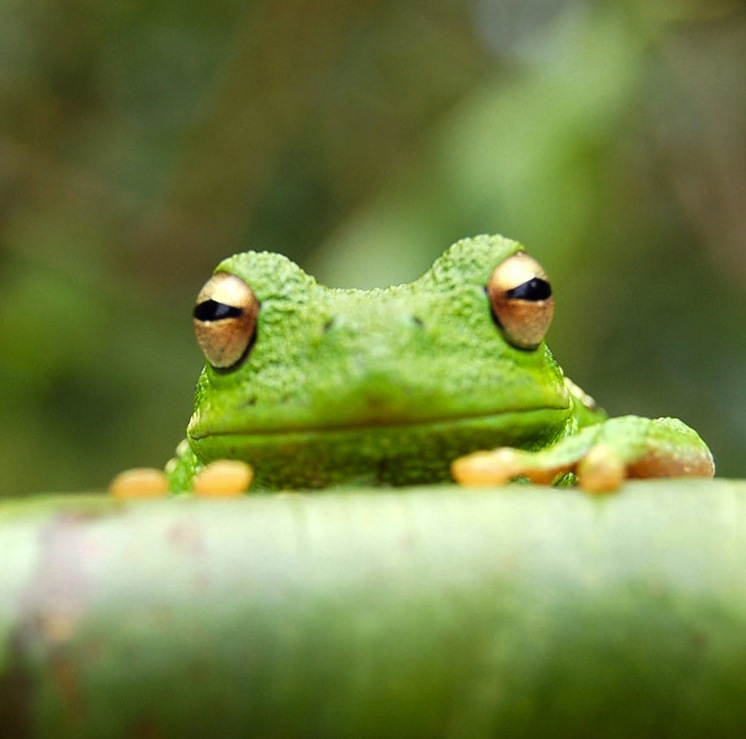
\includegraphics[width=0.40\textwidth]{frog.jpg} %{imagem} %extensões: .pdf, .png, .jpeg 
    %        [width=5cm]
    \caption{Caption - legenda da figura.\label{fig:imagem}}
    
\end{figure}

Na Figura~\ref{fig:imagem} (página?) podemos observar...

\chapter{Grafos}

\section{incluir imagens}

\subsection{grafo 01} \label{subsec:g01} 
\begin{figure}[hbt]
    \centering
    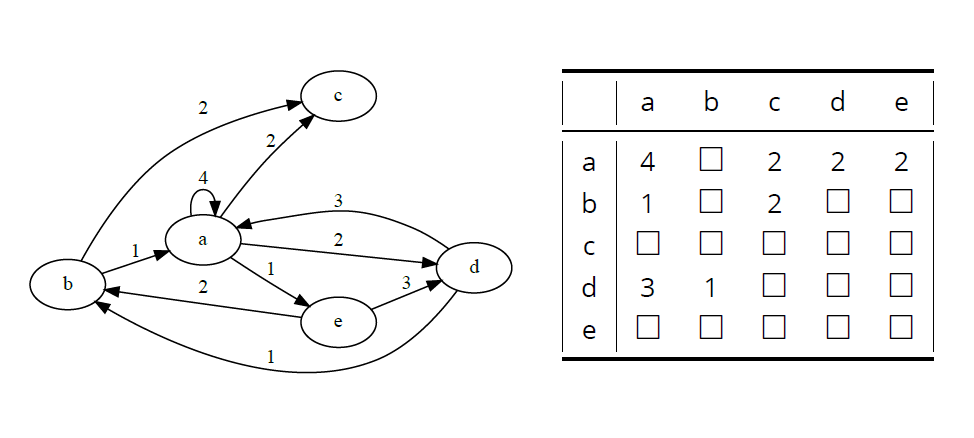
\includegraphics[width=0.6\textwidth]{grafo-d-matrizadj.PNG} 
    \caption{grafo pesado e orientado (digraph).\label{fig:grafo-d}}  
\end{figure}

Na Figura~\ref{fig:grafo-d}  (ver subsecção~\ref{subsec:g01})


% -------------------------------
\subsection{grafo 02}
\begin{figure}[h!bt]
    \centering
    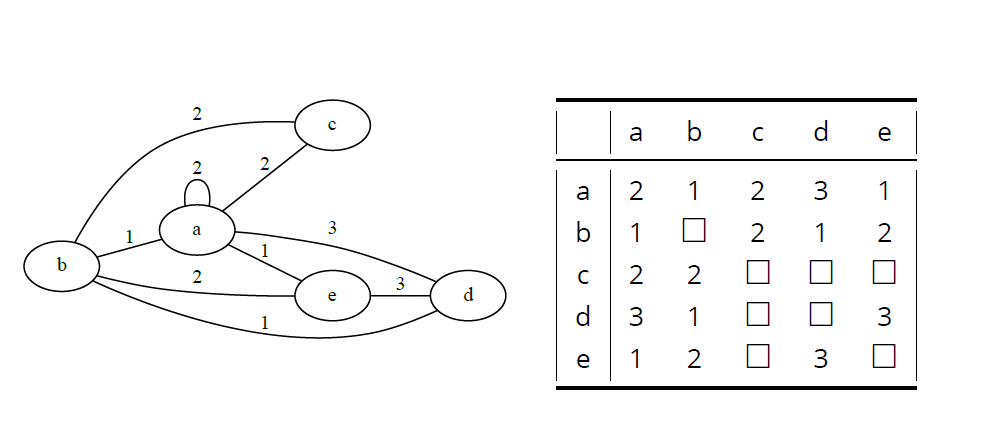
\includegraphics[width=0.60\textwidth]{grafo-matrizadj.PNG} 
    \caption{grafo pesado não orientado. \label{fig:grafo}}
\end{figure}

Na Figura~\ref{fig:grafo}

\section{tabular (para matriz)}

\begin{table}[h]
    \centering
    \begin{tabular}{|l|c|r|}
        \hline
        X  & = & X+1 \\
        \hline
        10 & = & 11 \\
        \hline
    \end{tabular}
    \caption{legenda da tabela. }
    \label{tab:exemplo}
\end{table}
Na Tabela~\ref{tab:exemplo}
    
\begin{table}[h]
    \centering
     \begin{tabular}{|c|ccccc|}
        \hline
        & a & b & c & d & e \\
        \hline
        a & 4 & $\ $ & 2 & 2 & 2 \\
        b & 1 & $\ $ & 2 & $\ $ & $\ $ \\
        c & $\ $ & $\ $ & $\ $ & $\ $ & $\ $ \\
        d & 3 & 1 & $\ $ & $\ $ & $\ $ \\
        e & $\ $ & $\ $ & $\ $ & $\ $ & $\ $\\
        \hline
      \end{tabular}
    \caption{legenda da tabela. }
    \label{tab:exemplo}
\end{table}


\begin{table}[htb]
    \centering
    \begin{tabular}{|cccc|c|}
        \hline
        \textbf{A} & \textbf{B} & 
        \textbf{C} & \textbf{D} & \textbf{Total} \\
        \hline
          1 & 2 & 3 & 4 & 10  \\
          2 & 3 & 4 & 5 & 14  \\
          3 & 4 & 5 & 6 & 18  \\
          4 & 5 & 6 & 7 & 22 \\
          \hline
    \end{tabular}
    \caption{Legenda da tabela.}
    \label{tab:1}
\end{table}
\section{graphviz (para desenhar o grafo)}
%\usepackage[pdf]{graphviz}
\begin{figure}
    \centering
    %[scale=0.45]
    \digraph[scale=0.45]{abc7}{
        rankdir=LR;
        ranksep=0.5;
        %origem -> destino [label=peso]
        b->a [label=100]; 
        b->c [label=2];
        a->a [label=4];
        d->a [label=3];
        a->d [label=2];
        d->b [label=1];
        e->b [label=2];
        e->d [label=3];
        a->c [label=2];
        a->e [label=1];
      }      
    \caption{grafo resultado. \label{fig:grafo-d}}
\end{figure}

\subsection{implementação em C}

\subsubsection{Adjacency Matrices}
  \begin{itemize}
  \item Useful if number of vertices is known;
  \item If there is a high number of vertices but a few edges, the
    matrix is too sparse (too much wasted space);
  \item For small graphs or highly connected graphs it can be highly
    efficient.
  \end{itemize}


  A simple approach:
  \begin{lstlisting}
#define N 100

float graph[N][N];    
\end{lstlisting}

Problem:
\begin{itemize}
\item How to represent a non existing connection?
  \begin{itemize}
  \item If there are no 0-weighted edges, use the 0;
  \item You can use NAN (\verb!math.h!);
  \end{itemize}
\end{itemize}

\subsection{matriz de adjacência}  

A implementação da função para inicializar o grafo vazio é apresetada na Listagem~\ref{lst:1}: 
\begin{lstlisting}[caption={inicializar o grafo vazio},
                   label=lst:1]
   void init_graph(float g[N][N]) {
      for (int i = 0; i < N; ++i)
        for (int j = 0; j < N; ++j)
          g[i][j] = NAN;
    }
\end{lstlisting}

Inicializar o grafo como vazio:

  \begin{lstlisting}
    
  \end{lstlisting}

Adicionar um arco

  \begin{lstlisting}
 void add_edge(float g[N][N], int f, int t, float w) {
    g[f][t] = w;
 }
  \end{lstlisting}
Verificar a existencia de um arco
  \begin{lstlisting}
 int has_edge(float g[N][N], int f, int t) {
    return !isnan(g[f][t]));
 }
  \end{lstlisting}
  
Obter o peso de um dado arco:
    \begin{lstlisting}
float edge_weight(float g[N][N], int f, int t) {
    return g[f][t];
 }
  \end{lstlisting}




\chapter{Conclusão} 
\label{cap:conclusao} % uma referência para o capítulo Conclusão
%\section{Conclusão}
A conclusão do documento...

\section{principais contributos do trabalho}
Este projeto encontra-se descrito na sua página web 
%\url{http://www.projeto.pt} % necessário \usepackage{url}
\footnote{página do projeto: \url{http://www.projeto.pt}}

\section{principais dificuldades}

\section{indicar as mais valias do trabalho}

\end{document}
